\chapter{Implementation And Visual Interface}
\label{ch:implementation}

The theoretical analysis presented in the preceding chapters establish the mathematical and historic background of the \texttt{DIJKSTRA-PREDICTION} algorithm. The following two chapters aim to help readers understand the computational strength and practical limitations of the algorithm.

We split our contributions in two parts:
\begin{enumerate}
    \item Chapter \ref{ch:implementation}, which details the front-end interactive webpage, back-end algorithmic logic and integration of the \texttt{DIJKSTRA-PREDICTION} algorithm, as well as \texttt{DIJKSTRA} and other traditional based ML approaches, providing a visualization framework in real-time.
    \item Chapter \ref{ch:experimentation}, which aims to showcase the same algorithms across many large-scale graphs and targeted graph topologies to demonstrate the efficiency of \texttt{DIJKSTRA-PREDICTION}.
\end{enumerate}
Furthermore, in Chapter \ref{ch:implementation} we have:
\begin{itemize}
    \item Section \ref{sec:frontend}, which describes in detail and provides screenshots on the front-end of the interface (\textit{UI/UX, design, etc.})
    \item Section \ref{sec:backend}, which goes over the back-end functionality of the interface and the implementation of each algorithm.
\end{itemize}

\section{The Interactive Visual Environment} \label{sec:frontend}
The Visual Environments consists of a custom full-stack web application. This interactive visualizer acts as a tool for creating/editing/generating complex graphs and testing the \texttt{DIJKSTRA-PREDICTION} algorithm alongside \texttt{DIJKSTRA} and traditional machine learning models. The application also provides a step-by-step animation of the algorithms (including the priority queue operations). It is structured in a React-based front-end engine and a Python-based back-end algorithm with REST API.

\subsection{Front-end Architecture and Graph Rendering}
\label{subsec:frontend}
The primary interface consists of an vast, interactive 2D canvas, implemented with React Flow, where users have the ability to dynamically construct graphs anywhere on the workspace and establish directed edges between them\footnote{A user may use two directed edges in the opposite direction for undirected logic.}. Users may create a graph of with any amount of nodes and edges they want (See Figure \ref{fig:main_canvas}).

\begin{figure}[htbp]
    \centering
    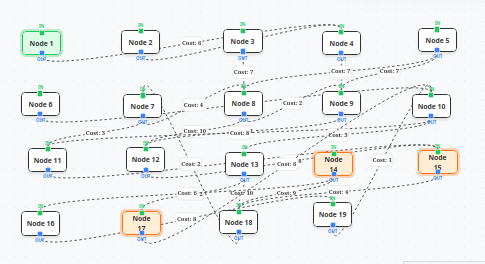
\includegraphics[width=0.9\textwidth]{images/random_graph.png}
    \caption{The main interactive canvas of the visualizer, displaying a randomly generated graph topology with explicit nodes, directional edges, and assigned computational costs.}
    \label{fig:main_canvas}
\end{figure}
\vspace{2cm}

\subsection{Toolkit and Node State Representation}

The environment also features a toolbar (Graph Tools), which dynamically adapts its available actions based on the user's element selection:

\begin{figure}[htbp]
    \centering
    \begin{minipage}{0.45\textwidth}
        \centering
        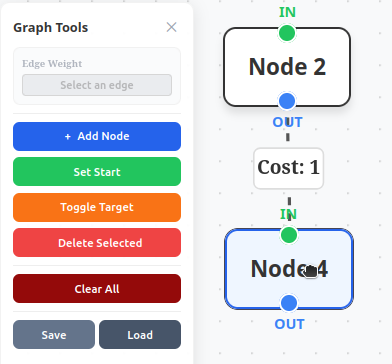
\includegraphics[width=0.8\textwidth]{images/graph_tools_selected_node.png}
        \caption{Toolbar options available when a node is actively selected.}
        \label{fig:tools_node}
    \end{minipage}\hfill
    \begin{minipage}{0.45\textwidth}
        \centering
        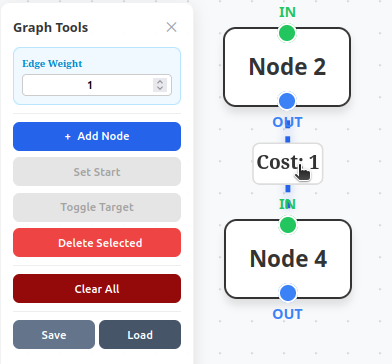
\includegraphics[width=0.8\textwidth]{images/graph_tools_selected_edge.png}
        \caption{Toolbar options available when an edge is actively selected.}
        \label{fig:tools_edge}
    \end{minipage}
\end{figure}

\begin{itemize}
    \item When a \textit{node} is selected the toolbar activates specific controls allowing the user to change the designated role of a node (See Figure \ref{fig:tools_node}). Users can set a unique starting point (\texttt{Set Start}), mark it as one of the multiple targets (\texttt{Toggle Target}), or remove it entirely (\texttt{Delete Selected}). Furthermore, the state of a node can also be alter by the underlying algorithm being run. For example a \textbf{Visited Node} will appear different to a \textbf{Path Node}. This visual distinction is necessary in order to distinguish between nodes that were explored and nodes that were permanently settled (See Figure \ref{fig:node_states}). 
    \begin{figure}[h]
        \centering
        \begin{subfigure}[b]{0.3\linewidth}
            \centering
            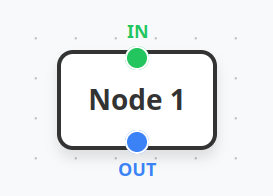
\includegraphics[width=\linewidth]{tex/images/node_simple.png}
            \caption{Neutral State}
            \label{subfig:simple}
        \end{subfigure}
        \hfill
        \begin{subfigure}[b]{0.3\linewidth}
            \centering
            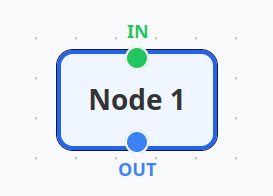
\includegraphics[width=\linewidth]{tex/images/node_selected.png}
            \caption{Selected State}
            \label{subfig:selected}
        \end{subfigure}
        \hfill
        \begin{subfigure}[b]{0.3\linewidth}
            \centering
            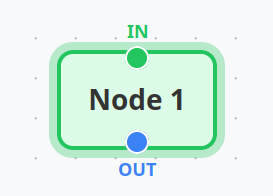
\includegraphics[width=\linewidth]{tex/images/node_start.png}
            \caption{Start State}
            \label{subfig:start}
        \end{subfigure}
        \begin{subfigure}[b]{0.3\linewidth}
            \centering
            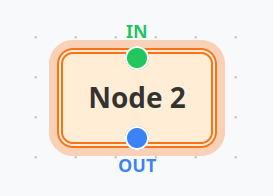
\includegraphics[width=\linewidth]{tex/images/node_target.png}
            \caption{Target State}
            \label{subfig:target}
        \end{subfigure}
        \hfill
        \begin{subfigure}[b]{0.3\linewidth}
            \centering
            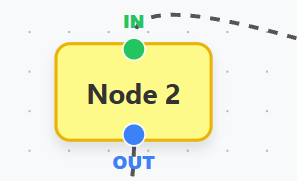
\includegraphics[width=\linewidth]{tex/images/node_pq.png}
            \caption{Priority Queue State}
            \label{subfig:prio-queue}
        \end{subfigure}
        \hfill
        \begin{subfigure}[b]{0.3\linewidth}
            \centering
            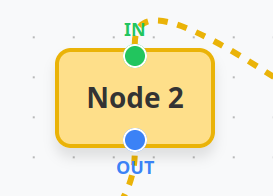
\includegraphics[width=\linewidth]{tex/images/node_visited.png}
            \caption{Visited State}
            \label{subfig:visited}
        \end{subfigure}
        \begin{subfigure}[b]{0.3\linewidth}
            \centering
            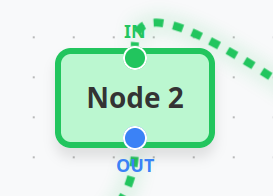
\includegraphics[width=\linewidth]{tex/images/node_path.png}
            \caption{Path State}
            \label{subfig:path}
        \end{subfigure}
        
        \caption{Visual vocabulary for node states. The color-coded system tracks a node's "status" during execution, distinguishing between unexplored, active priority queue frontiers, settled nodes, and the final optimal path.}
        \label{fig:node_states}
    \end{figure}
    \vspace{5cm}

    \item When an \textit{edge} is selected (See Figure \ref{fig:tools_edge}), the toolbar activates an \texttt{Edge Weight} input space, allowing the user to edit the value of the selected edge's weight. Similar to the nodes, the corresponding color of an edge may change depending on its state while and after running an algorithm (See Figure \ref{fig:edge_legend}).
    \begin{figure}
        \centering
        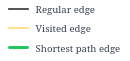
\includegraphics[width=0.3\linewidth]{tex/images/edge_legend.png}
        \caption{Visual representation of edge states. Similar to nodes, edges dynamically update their color, highlighting their role during and after execution.}
        \label{fig:edge_legend}
    \end{figure}
\end{itemize}
\vspace{1cm}
\newpage

To further enhance user experience, the visualizer enables the user with global topology management actions (See Figure \ref{fig:graph_actions}). Users can completely clear the canvas by utilizing \texttt{Clear All} function, save or load\footnote{This function is achieved by utilizing the browser's native File API to package the graph state and trigger a local file download} specific user built graphs as a JSON object to local storage using the \texttt{Save}/\texttt{Load} functionality, or instantly generate a \texttt{Random Graph}, or a Pre-Built \texttt{Trap Scenario} (See Section \ref{subsec:trap}) which showcases the advantage of \texttt{DIJKSTRA-PREDICTION}. 


\begin{figure}[htbp]
    \centering
    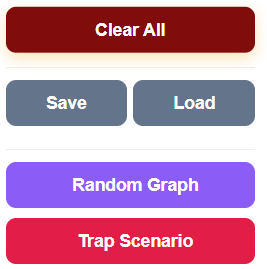
\includegraphics[width=0.4\textwidth]{tex/images/graph_tools_graph_actions.png}
    \caption{The global graph management toolkit. These controls allow users to load or save the current topology of any graph in their local files, clear and reset the 2d canvas, or generate a random graph topology or trap scenario (based on internal rules).}
    \label{fig:graph_actions}
\end{figure}

Furthermore, as user generated graphs may grow in scale and complexity, navigating an expanding 2D canvas may become quite challenging. To combat this issue, the visualizer uses a suite of view-port controls. Users can dynamically pan and adjust the zoom level of the workspace\footnote{Can also be controlled with the mouse using the scroll wheel.}, lock the interactivity with the graph or even automatically fit the graph in view (See Figure \ref{fig:view_utils}). User can also utilize a mini-map to have a quick grayscale view of the environment and help traverse it instantly (see Figure \ref{fig:minimap})


\begin{figure}[h]
    \centering
    \begin{subfigure}[b]{0.23\linewidth}
        \centering
        
\includegraphics[height=\linewidth]{tex/images/enviroment_tools.png}
        \caption{View-port}
        \label{subfig:simple}
    \end{subfigure}
    \hfill
    \begin{subfigure}[b]{0.36\linewidth}
        \centering
        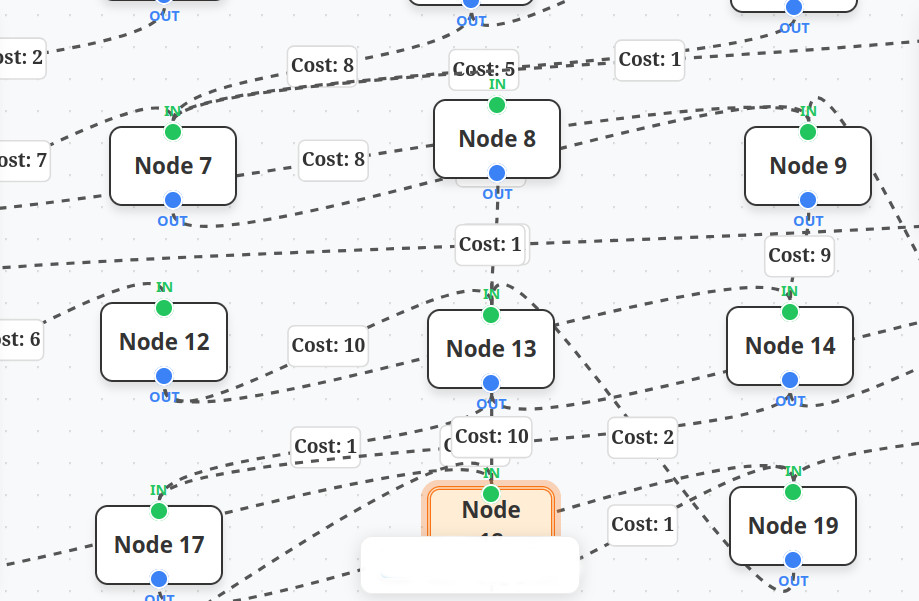
\includegraphics[width=\linewidth]{tex/images/before_fit.jpg}
        \caption{Starting View}
        \label{subfig:selected}
    \end{subfigure}
    \hfill
    \begin{subfigure}[b]{0.36\linewidth}
        \centering
        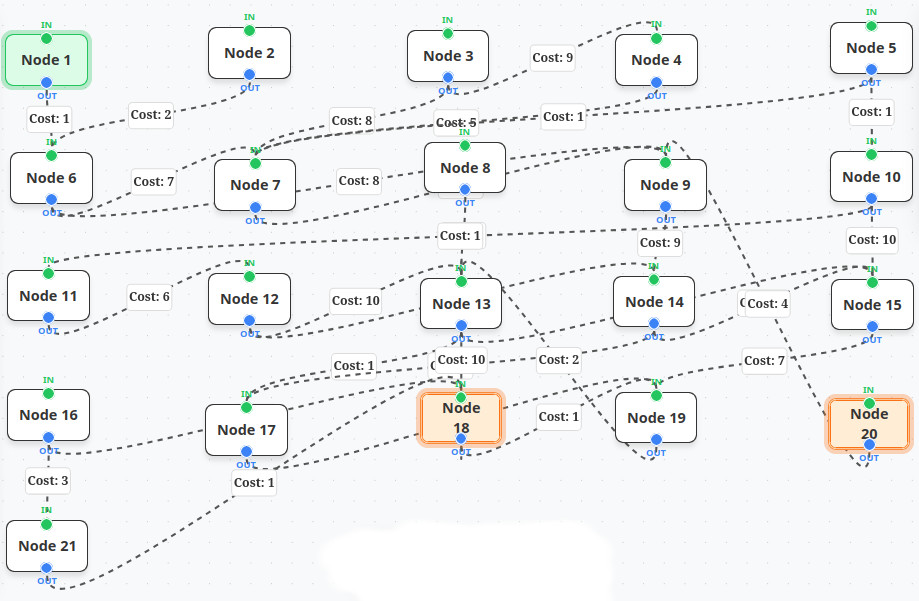
\includegraphics[width=\linewidth]{tex/images/after_fit.jpg}
        \caption{After Fit View}
        \label{subfig:start}
    \end{subfigure}
    \caption{Demonstration of the view-port controls. Utilizing the "Fit-to-Screen" functionality allows the user to instantly readjust the canvas from a tightly zoomed-in section (b) to a comprehensive, centered overview of the entire graph topology (c).}
    \label{fig:view_utils}
\end{figure}

\begin{figure}
    \centering
    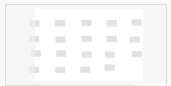
\includegraphics[width=0.5\linewidth]{tex/images/minimap.png}
    \caption{The dynamic minimap interface. This component provides an overview of the 2D canvas, ensuring users maintain awareness and control.}
    \label{fig:minimap}
\end{figure}
\vspace{10cm}


\subsection{Trap Scenario}
\label{subsec:trap}

As depicted in Figure \ref{fig:trap_scenario_canvas}, this pre-built scenario consists of a low-cost linear path leading towards the target, which eventually branches out into multiple high-cost dead-ends (traps). This topology is specifically generated by the visualizer to highlight the differences between \texttt{DIJKSTRA} and \texttt{DIJKSTRA-PREDICTION}.

\begin{figure}[htbp]
    \centering
    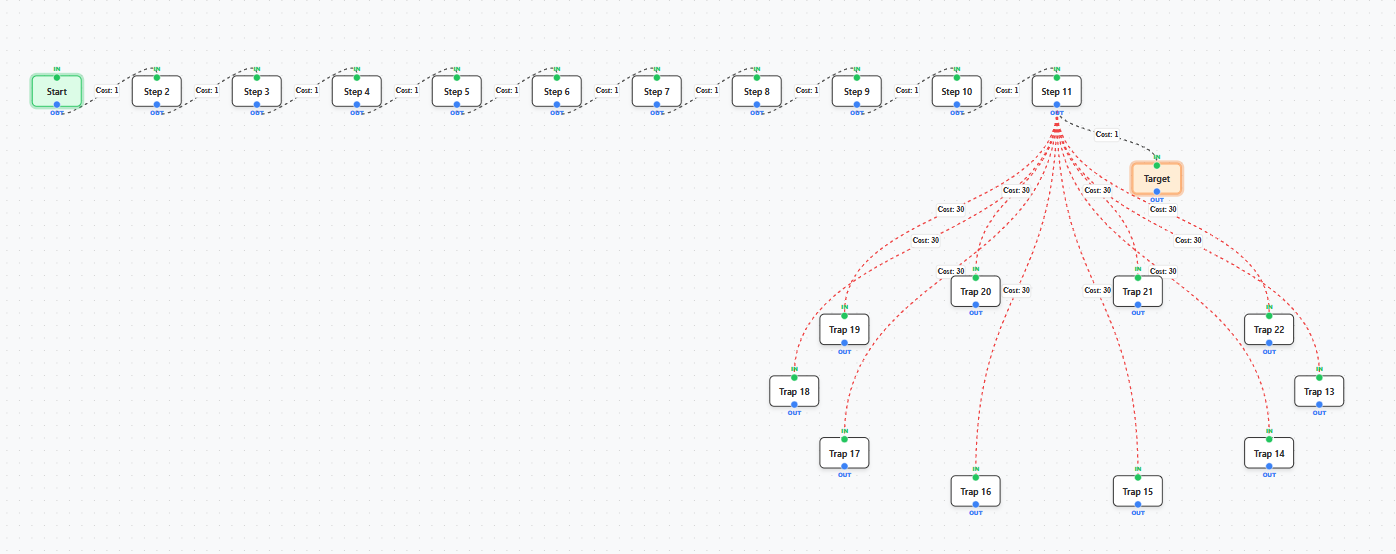
\includegraphics[width=\textwidth]{images/trap_scenario.png}
    \caption{The Pre-Built Trap Scenario topology generated by the visualizer. High-cost trap nodes branch out near the target to highlight the pruning efficiency of the learning-augmented approach.}
    \label{fig:trap_scenario_canvas}
\end{figure}

To demonstrate the difference, users may executes both algorithms on this trap scenario. Figure \ref{fig:trap_comparison} provides a visual comparison of the two algorithms.

When \texttt{DIJKSTRA} reaches the branching node, its exploration mechanism cause all \textit{trap} nodes to be inserted into the priority queue, thus wasting time executing actions.

On the other hand, \texttt{DIJKSTRA-PREDICTION} manages to compute a $P$ threshold value by step $i_0 = 10$ effectively pruning all trap nodes and saving on computational cost.
\newpage

\begin{figure}[htbp]
    \centering
    \begin{subfigure}[b]{0.48\textwidth}
        \centering
        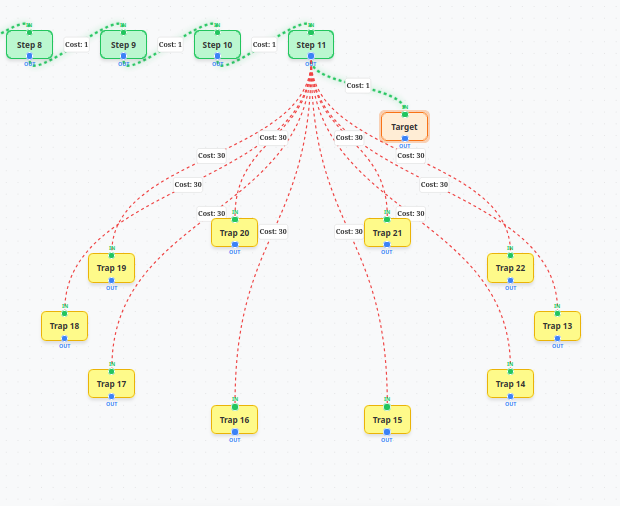
\includegraphics[width=\linewidth]{tex/images/trap_dijkstra.png}
        \caption{\textsc{DIJKSTRA}: All trap nodes are inserted into the search frontier, causing unnecessary priority queue actions.}
        \label{subfig:trap_dijkstra}
    \end{subfigure}
    \hfill
    \begin{subfigure}[b]{0.48\textwidth}
        \centering
        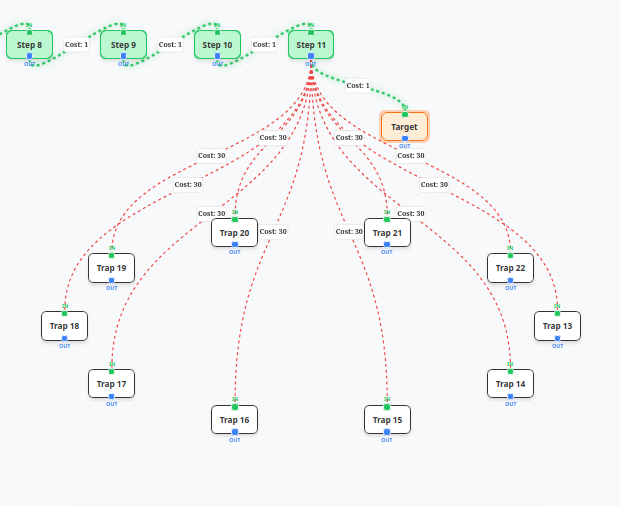
\includegraphics[width=\linewidth]{tex/images/trap_dijkstra_pred.png}
        \caption{\textsc{DIJKSTRA-PREDICTION}: Trap nodes are successfully pruned by utilizing a prediction threshold.}
        \label{subfig:trap_pred}
    \end{subfigure}
    \caption{Comparative execution of the Trap Scenario. }
    \label{fig:trap_comparison}
\end{figure}


\subsection{In-App Documentation and Notes}
\label{subsec:info}

For the purposes of transparency the application provides documentation and notes via a "Info" button located within the view-port controls toolkit (Figure \ref{subfig:info_button}).

Activating this toggle overlays a panel directly onto the workspace (Figure \ref{subfig:info_panel}). The panel contains info, setups, as well as findings, all together with a direct link to this thesis paper to help guide users.

\begin{figure}[htbp]
    \centering
    \begin{subfigure}[b]{0.15\textwidth}
        \centering
        
\includegraphics[width=\linewidth]{tex/images/info_button.png}
        \caption{Info Button}
        \label{subfig:info_button}
    \end{subfigure}
    \hfill
    \begin{subfigure}[b]{0.75\textwidth}
        \centering
        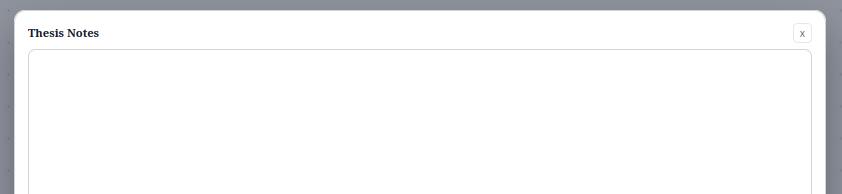
\includegraphics[width=\linewidth]{tex/images/info_panel.jpg}
        \caption{Thesis Notes Panel}
        \label{subfig:info_panel}
    \end{subfigure}
    \caption{The in-app documentation utility. The contextual Info button (a) activates the Thesis Notes modal (b), providing a unified interface for logging experimental observations and theoretical parameters.}
    \label{fig:info_feature}
\end{figure}


\subsection{Algorithm Selection}
\label{subsec:algorithm_selection}
The user has the ability to select which algorithm to execute. This is enabled through a drop-down selection interface on the toolbar (Graph Tools), See Figure \ref{fig:run_algorithms}.

\begin{figure}[htbp]
    \centering
    \begin{subfigure}[b]{0.45\textwidth}
        \centering
        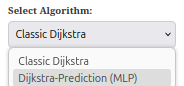
\includegraphics[width=0.7\linewidth]{tex/images/dropdown_closed.png}
        \caption{Expanded Drop-down Menu}
        \label{subfig:menu_expanded}
    \end{subfigure}
    \hfill
    \begin{subfigure}[b]{0.45\textwidth}
        \centering
        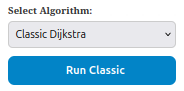
\includegraphics[width=0.7\linewidth]{tex/images/dropdown_open.png}
        \caption{Active Selection and Execution}
        \label{subfig:menu_execution}
    \end{subfigure}
    \caption{The algorithm selection interface. Users can expand the menu to choose between models (a). Once selected, the execution button triggers the backend processing (b).}
    \label{fig:run_algorithms}
\end{figure}

Upon clicking \texttt{Run}, the front-end process prepares the graph. It packages the topology into a structured JSON payload. This payload is then transmitted to the back-end to be processed. 


\subsection{The Playback Engine and State Management}
\label{subsec:playback_engine}

When the back-end returns the execution history (\texttt{visited\_steps} and \newline \texttt{queue\_steps}), a \texttt{buildTimeline} function executes. 

The animation is driven by (\texttt{currentStep}) and a timer. As the timer passes, the \texttt{applyStep} function modifies the CSS classes of the React Flow elements, visually distinguishing the priority queue without modifying the graph data structure.

To showcase the process, Figure \ref{fig:playback_sequence} demonstrates a step-by-step execution of the classic \textsc{DIJKSTRA} algorithm. Nodes and edges swap through node states (See Figures \ref{fig:node_states} and \ref{fig:edge_legend}) based on the back-end. Initially, neighbors of the active node are inserted into the \textit{priority queue}. In the  frames, nodes are extracted from the \textit{priority queue} and marked as permanently visited. Upon reaching the target, the engine solves the \texttt{paths} array from the payload, highlights the final optimal route.

\begin{figure}[h]
    \centering
    \begin{subfigure}[b]{0.35\textwidth}
        \centering
        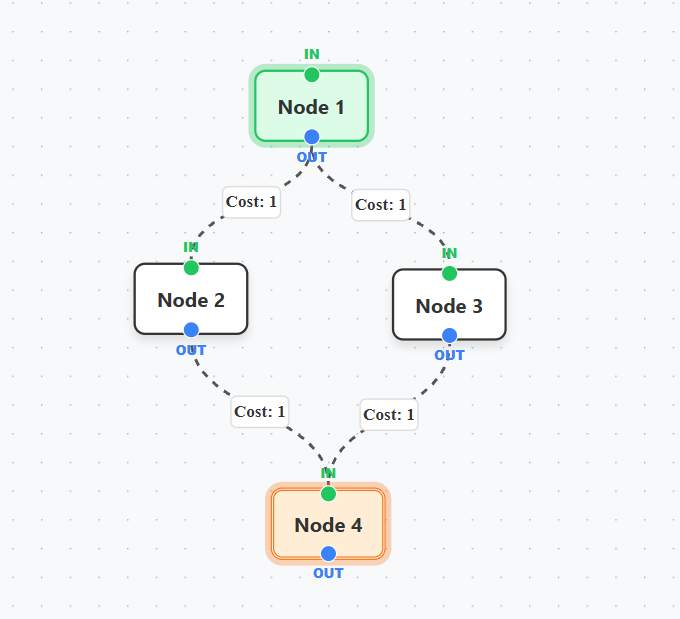
\includegraphics[width=\linewidth]{tex/images/run_step_1.png}
        \caption{Starting state of the graph. All nodes remain unexplored.}
        \label{subfig:step1}
    \end{subfigure}
    \hfill
    \begin{subfigure}[b]{0.35\textwidth}
        \centering
        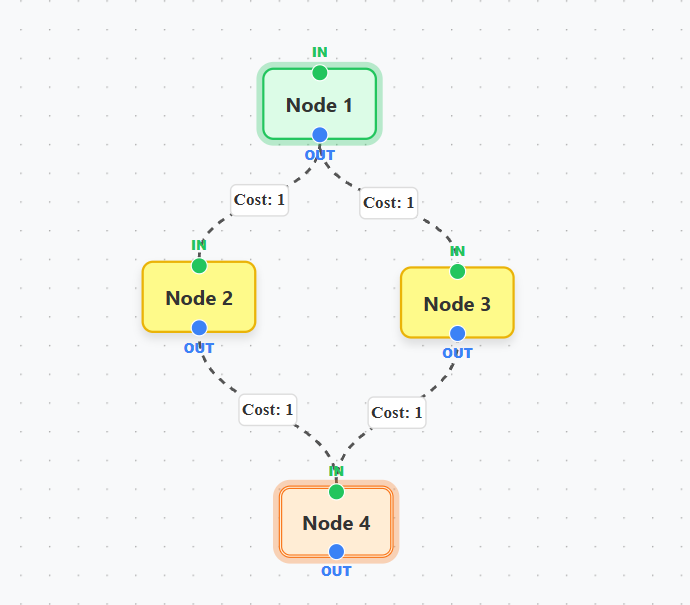
\includegraphics[width=\linewidth]{tex/images/run_step_2.png}
        \caption{Neighbors of the start node are inserted into the priority queue.}
        \label{subfig:step2}
    \end{subfigure}
    
    \begin{subfigure}[b]{0.35\textwidth}
        \centering
        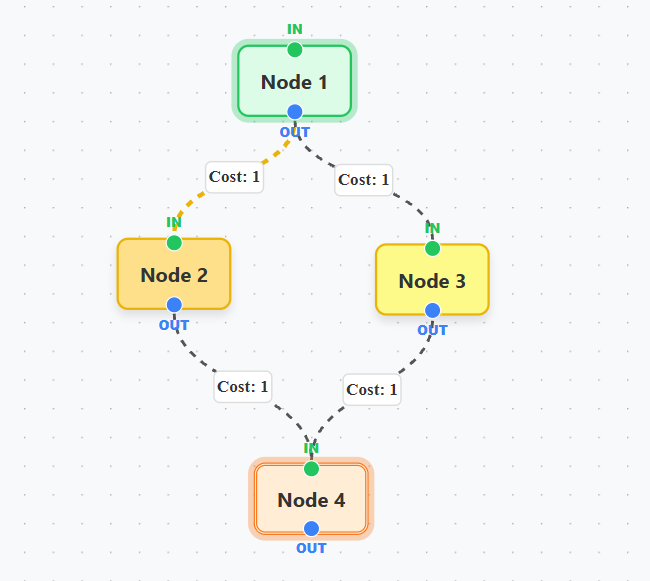
\includegraphics[width=\linewidth]{tex/images/run_step_3.png}
        \caption{ A node is extracted from the queue (visited).}
        \label{subfig:step3}
    \end{subfigure}
    \hfill
    \begin{subfigure}[b]{0.35\textwidth}
        \centering
        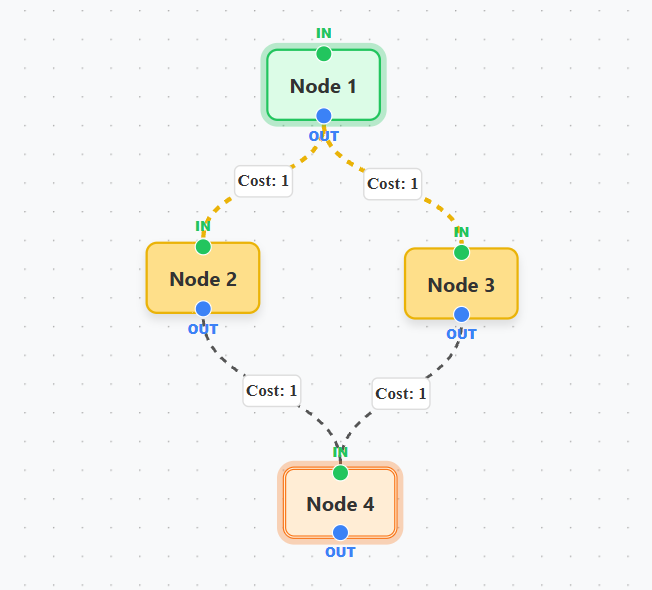
\includegraphics[width=\linewidth]{tex/images/run_step_4.png}
        \caption{The algorithm continues exploring nodes in the queue.}
        \label{subfig:step4}
    \end{subfigure}
    \caption{Sequential playback of the classic \textsc{DIJKSTRA} algorithm. The playback engine updates the visual state of nodes and edges at each time step.}
    \label{fig:playback_sequence}
\end{figure}

The logic of the playback engine relies on two primary procedures (Algorithms \ref{alg:build_timeline} and \ref{alg:apply_step}). The \textsc{BUILD-TIMELINE} algorithm processes the raw execution trace. By checking the state of the priority queue at each step, it filters out redundant operations (e.g. No changes in priority queue) and constructs a sequence of animation frames, without duplicates. 

The \textsc{APPLY-STEP} algorithm take care of the visual rendering. Given a specific frame from the timeline, it resets the canvas and applies the correct CSS classes based on the previously states Node and Edge States (See Figures \ref{fig:node_states} and \ref{fig:edge_legend}). The algorithm transitions nodes between the \textit{priority queue} state and the \textit{visited} state. When the timeline reaches the final "path" frame, it highlights the final optimized shortest path.
\vspace{0.5cm}

\begin{algorithm}[H]
\caption{BUILD-TIMELINE(data)} \label{alg:build_timeline}
$timeline = []$\;
$lastQueueKey = null$\;

\ForEach{$step$ \textnormal{in} $data.visited\_steps$}{
    $i = \textnormal{index of } step$\;
    $queueSnapshot = \textnormal{GET-SNAPSHOT}\footnote{Explanation on State Snapshots on Section \ref{subsec:state_snapshots}}(data.queue\_steps, i)$\;
    $queueKey = \textnormal{HASH}(queueSnapshot)$ \tcp*{generate unique state key}
    
    \If{$queueKey \neq lastQueueKey$}{\tcp{only add to timeline if there's a change}
        $timeline\textnormal{.APPEND}(\{type: \text{"queue"}, index: i\})$ \tcp*{record queue update}
        $lastQueueKey = queueKey$\;
    }
    $timeline\textnormal{.APPEND}(\{type: \text{"visit"}, index: i+1\})$ \tcp*{record node visit}
}

$timeline\textnormal{.APPEND}(\{type: \text{"path"}\})$ \tcp*{final resolution step}
\Return $timeline$\;
\end{algorithm}

\begin{algorithm}[H]
\caption{APPLY-STEP(timelineIndex, data, timeline)} \label{alg:apply_step}
RESET-VISUAL-STATES() \tcp*{clear all visual node/edge classes}
$step = timeline[timelineIndex]$\;

\eIf{$step.type == \text{"path"}$}{
    HIGHLIGHT-ALL($data.visited\_steps$, "visited")\;
    HIGHLIGHT-PATH($data.paths$, "path-node") \tcp*{highlight optimal route}
    UPDATE-UI-STATS($data.queue\_steps[-1]$) \tcp*{display final P and B}
}{
    $i = step.index$\;
    $visitedSet = \textnormal{GET-VISITED-UNTIL}(data.visited\_steps, i)$\;
    $queueSet = \textnormal{GET-QUEUE-SNAPSHOT}(data.queue\_steps, i)$\;

    \If{$step.type == \text{"visit"}$}{
        $queueSet\textnormal{.REMOVE}(data.visited\_steps[i])$ \tcp*{node transitions to visited}
    }

    HIGHLIGHT-NODES($visitedSet$, "visited")\;
    HIGHLIGHT-NODES($queueSet$, "queue-node")\;
    UPDATE-UI-STATS($data.queue\_steps[i]$) \tcp*{update real-time P and B}
}
\end{algorithm}
\vspace{0.5cm}


\subsection{Animation Controls}
\label{subsec:navigation_animation}
To give users full control over the playback engine rather than automatically and instantaneously rendering the final shortest path, the environment by default is designed to automatically execute the \texttt{applyStep} updates with a timed delay (\textit{1000ms/1s}), and even further provides the user with an interactive bottom toolkit for \texttt{Pause} and \texttt{Play} functionality, as well as \texttt{Next Step} and \texttt{Previous Step} options (See Figure \ref{fig:animation_tools}).

\begin{figure}[htbp]
    \centering
    
\includegraphics[width=0.5\linewidth]{tex/images/animation_tools.png}
    \caption{Interactive animation playback controls. This toolkit enables, frame-by-frame traversal of the algorithm's execution history.}
    \label{fig:animation_tools}
\end{figure}

\section{Backend Architecture and API Design}
\label{sec:backend}

The back-end of the visualizer is developed using Python and specifically \texttt{FastAPI}. This framework was selected for its performance and support for REST (Representational State Transfer) APIs. To allow secure, cross-domain communication, we utilise Cross-Origin Resource Sharing (CORS), preventing cross-site suspicious request.

\subsection{Data Validation and Payload Structure}
\label{subsec:data_validation}

We ensure that the graph created by the user in the React front-end environment is correctly processed through data validation. We achieve this by utilizing \texttt{Pydantic} models. 

\begin{itemize}
	\item The system defines an \texttt{EdgeModel} class to correctly store all useful information about an edge (\texttt{source}, \texttt{target}, and \texttt{weight}). 
	\item The \texttt{GraphPayload} defines the JSON structure of the incoming request, containing the \texttt{startNode}, a list of \texttt{targetNodes}, and the complete arrays of nodes and edges.
\end{itemize}

\subsection{The Endpoint Communication}
\label{subsec:solver_endpoint}

The communication between the front-end and back-end occurs through a single \texttt{POST} endpoint denoted as \texttt{/solve}. Upon receiving a request, the back-end parses the JSON payload into the \texttt{GraphPayload} model we saw before. 

The Endpoint then precedes to execute the algorithms \texttt{DIJKSTRA} and \texttt{DIJKSTRA-PREDICTION}, one after the other, on the same graph data. After executing the endpoint bundles the result (i.e. the \texttt{visited\-steps} and \texttt{queue\-steps} arrays). After this response reaches the front-end it can be processed by the playback engine to deliver the animation to the user depending on the algorithm chosen (See Section \ref{subsec:algorithm_selection})

\subsection{Algorithmic Translation and State Snapshots}
\label{subsec:state_snapshots}
The algorithms, \texttt{DIJKSTRA} and \texttt{DIJKSTRA-PREDICTION}, were both modified for the purpose of visualizing the results. A standard implementation would simply return the final optimal path found by the two algorithms, but for our goal we require a visualization of a \textit{snapshot} of the state of the nodes at every step of the algorithmic execution. 

Basically, as we stated before, our goal is to showcase the difference in the number of priority queue operations, which lead \texttt{DIJKSTRA-PREDICTION} to a faster running time. To achieve this, we utilize the Python \texttt{heapq} library, in order to mantain the priority queue data structure efficiently. At every step, the algorithms saves the exact state of the queue. For \texttt{DIJKSTRA-PREDICTION}, the algorithm also save the pruning bound ($B$).

\subsection{Oracle Integration and Data Structures}
\label{subsec:oracle_integration}

A big challenge when dealing with any algorithm with predictions is the integration of the machine learning oracle into the execution loop. The algorithm, \texttt{DIJKSTRA-PREDICTION} achieves this without an expensive computational cost through the use of the \texttt{joblib} library which loads the pre-trained model (Multi-Layer Perceptron - MLP) into the server's memory.

During the initial $i_0$ iterations of the algorithm, the back-end creates the trace by appending the lower bound $d_i$ together with the upper bound $B_i$ (See Section \ref{sec:dijkstra-prediction}) of each step. Once the trace is complete, it is formatted into a \texttt{NumPy} array and passed to the oracle to make a prediction $P$, for it to be used as a threshold. 

Lastly, the Reserve Set ($R$) was implemented using a Python hash map (dictionary), thus ensuring $O(1)$ execution time when executing any insertions, lookup and deletion. This allows the \texttt{UPDATE-PREDICTION} routine to be able to very quickly extract nodes from the Reserve Set ($R$) and re-insert them into the priority queue.

\subsection{Performance Tracking and Metrics Collection}
\label{subsec:performace_tracking}

Moving away from the visualization the backend collects data and metrics on the performance of the algorithms.

Because \textsc{DIJKSTRA-PREDICTION} maintains the  same complexity bound of $\mathcal{O}(m+n\log n)$ as classic \textsc{DIJKSTRA}, theoretical and visual analysis alone is not enough to evaluate its performance. Therefore, we utilize these metrics to accurately quantify the actual computational cost saved.

An optional \texttt{collect\_stats} parameter is integrated into the algorithm. When activated, it allows for tracking of every action with the data structures:


\begin{itemize}
    \item \textbf{Priority Queue Operations:} The algorithms record the number of insertions (\texttt{pq\_pushes}) and extractions (\texttt{pq\_pops}). They also track duplicate encounters (\texttt{pq\_skips}), which occur when a shorter path to an already enqueued node is discovered, bypassing unnecessary heap evaluations.
    \item \textbf{Reserve Set Operations:} Specific to \textsc{DIJKSTRA-PREDICTION}, the system logs the number of nodes pruned and stored in the fallback dictionary (\texttt{r\_inserts}), as well as the nodes recovered during an \texttt{UPDATE-PREDICTION} routine (\texttt{r\_rescues}).
\end{itemize}

Through this metrics, the algorithm allows us to move away from the theoretical background and claims in Chapter \ref{ch:learning_augmented}, and compare the results between \texttt{DIJKSTRA-PREDICTION}, \texttt{DIJKSTRA}, and other traditional Machine Learning approaches in Chapter \ref{ch:experimentation}.

\subsection{Full Overview of a Sequence Flow}
\label{subsec:sequence_flow}

To aid in the understanding of the synchronization between the front-end visual user interface and the back-end computational executions, we define the complete UML sequence diagram in Figure \ref{fig:uml_diagram}. 

\begin{figure}[h]
    \centering
    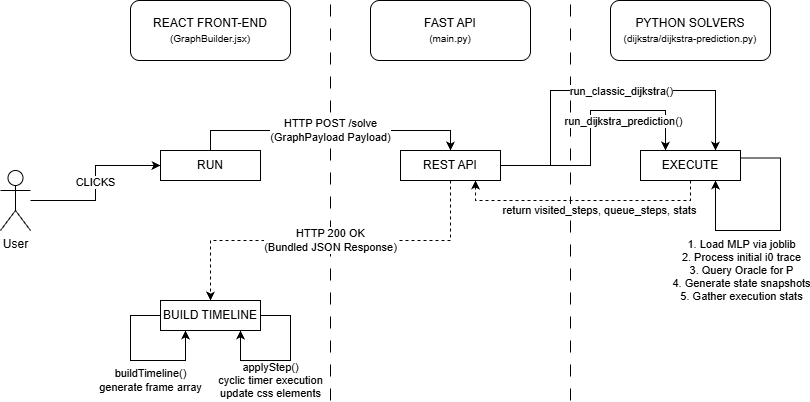
\includegraphics[width=1\linewidth]{tex/images/uml.drawio.png}
    \caption{UML Sequence Diagram illustrating the synchronous client-server execution loop. The front-end serializes the current canvas topology, which is then sequentially processed by both routing algorithms to extract performance metrics and step-by-step state animations.}
    \label{fig:uml_diagram}
\end{figure}

The diagram details the life cycle of a routing request. The operations pass through four different discrete phases:

\begin{enumerate}
    \item \textbf{React Front-End:} The process starts when the user presses on the execution button. The front-end packages the active nodes, directed edges, explicit weights, and multiple target states into a  structure following the \texttt{GraphPayload} Pydantic schema. This object is transmitted across domains via an HTTP \texttt{POST} request.
    \item \textbf{FastAPI Server:} Upon receipt, the \texttt{FastAPI} middleware performs schema validation. Only after passing validation does the server sequentially pass the computation to the algorithms.
    \item \textbf{Python Solvers:} The modules execute both classic \textsc{DIJKSTRA} and \textsc{DIJKSTRA-PREDICTION}. During execution, the internal states are recorded at every step, logging priority queue actions, reserve set operations, and specific bounding parameters ($B$ and $P$). Once finished, the execution data and performance metrics are packaged into a unified response payload.
    \item \textbf{Animation Playback:} The bundled JSON payload is returned to the client via an HTTP 200 OK response. The front-end playback engine receives this data, executes the \texttt{buildTimeline()} procedure to prune redundant frames where no changes occured, and begins the cyclic execution of \texttt{applyStep()} to update the visual states of the elements of the graph.
\end{enumerate}
 